\documentclass[11pt,a4paper]{article}
\usepackage[margin=1in]{geometry}
\usepackage{graphicx}
\usepackage{booktabs}
\usepackage{hyperref}
\usepackage{amsmath}
\usepackage{xcolor}
\usepackage{float}
\graphicspath{{../figures/}}

\title{Replication Report:\\Deep Learning of Atomically Resolved STEM Images\\\large OSTI ID 1427646}
\author{Automated replication (uicgpu, NVIDIA A100 80GB)}
\date{\today}

\begin{document}
\maketitle

\begin{abstract}
We replicate, at reduced but faithful scope, the pipeline of Ziatdinov \emph{et al.}
(OSTI 1427646) in which a fully convolutional neural network (FCN) performs
pixel-wise chemical identification of atomic columns in
SrTiO$_3$ / La$_{0.7}$Sr$_{0.3}$MnO$_3$ heterostructures imaged by HAADF-STEM.
Because experimental STEM stacks and full multislice simulations are out of
scope for a short replication, we build a physics-motivated synthetic surrogate:
perovskite [001] projected square lattices rendered as
Gaussian atomic columns with $Z^{1.7}$-weighted HAADF-like contrast,
interface diffuseness, Poisson counting noise, scan-line jitter, and random
defects (vacancies, A-site / B-site antisites). A 7.8\,M-parameter U-Net,
trained in 95\,s on one A100, recovers per-pixel class labels at
98.8\% accuracy and detects atomic columns with sub-pixel RMSE
(0.06--0.47 px at $\approx$0.2\,\AA/px, i.e. $\sim$10--100\,m\AA) and
$\geq 98\%$ recall across Sr, Ti, La/Sr, and Mn columns. These figures are
consistent with the paper's qualitative claim that a small FCN trained on
simulated data suffices for quantitative chemical mapping of perovskite
interfaces.
\end{abstract}

\section{Relationship to the original paper}
The original paper \cite{Ziatdinov2017} trains an encoder--decoder FCN on
\emph{multislice-simulated} HAADF-STEM images of perovskite heterostructures
and applies it to experimental data to produce per-column chemical labels,
atomic-position maps, and line-scan compositions across interfaces. The core
claim --- that a fully convolutional network trained purely on simulation
generalises well enough to assign chemical identities in real STEM data
--- rests on three operational ingredients: (i) realistic image formation,
(ii) a pixel-wise classifier with skip connections, and (iii) peak finding
on per-class probability maps.

This replication reproduces (ii) exactly (a small U-Net, 5 encoder stages,
skip connections, soft-max head), closely mirrors (iii) (connected-component
centroid finding on argmax maps), and \emph{substitutes} a lightweight
physics-motivated generator for (i). The substitution is deliberate: running
multislice with Prismatic/abTEM on tens of thousands of supercells exceeds
the 3-hour wall budget and is not the novel contribution of the paper. The
generator preserves the structural features the model would have to learn:
square A/B sublattices offset by $(a/2,a/2)$, $Z^{1.7}$ HAADF contrast,
A-site vs B-site intensity separation, scan-line distortion, and Poisson
noise.

\section{Methods}

\subsection{Synthetic STEM generator}
Each $256{\times}256$ frame represents roughly a $12 \times 12$ unit cell
perovskite [001] projection with $a \approx 20$\,px pitch (random 5\% jitter
per frame). The image has two horizontal regions --- SrTiO$_3$ (bottom) and
La$_{0.7}$Sr$_{0.3}$MnO$_3$ (top) --- separated by an interface at a
random $y$ with random diffuseness (0--1.5 unit cells, tanh-weighted mixing).
A-site and B-site columns are placed on two interleaved square sublattices
and rendered as Gaussian blobs ($\sigma \approx 3\,\text{px}$) with
intensities
\[
I_{\mathrm{Sr}} \propto 38^{1.7},\quad
I_{\mathrm{Ti}} \propto 22^{1.7},\quad
I_{\mathrm{La/Sr}} \propto 0.7\cdot 57^{1.7} + 0.3\cdot 38^{1.7},\quad
I_{\mathrm{Mn}} \propto 25^{1.7}.
\]
Per-column defects are drawn independently: vacancies (2\%) remove a column;
antisite defects (2\%) swap the cation identity so the network must learn
intensity, not position. Post-processing adds row-wise sub-pixel horizontal
jitter, Poisson counting at a peak of 400 counts, and small Gaussian
background noise. Labels are built as Gaussian footprints around each
column's $(x_c,y_c)$ and then argmaxed, so each pixel carries a single
class in $\{\text{vacuum},\text{Sr},\text{Ti},\text{La/Sr},\text{Mn},
\text{defect}\}$. Example inputs with ground-truth overlays appear in
Fig.~\ref{fig:data}.

\begin{figure}[H]
\centering
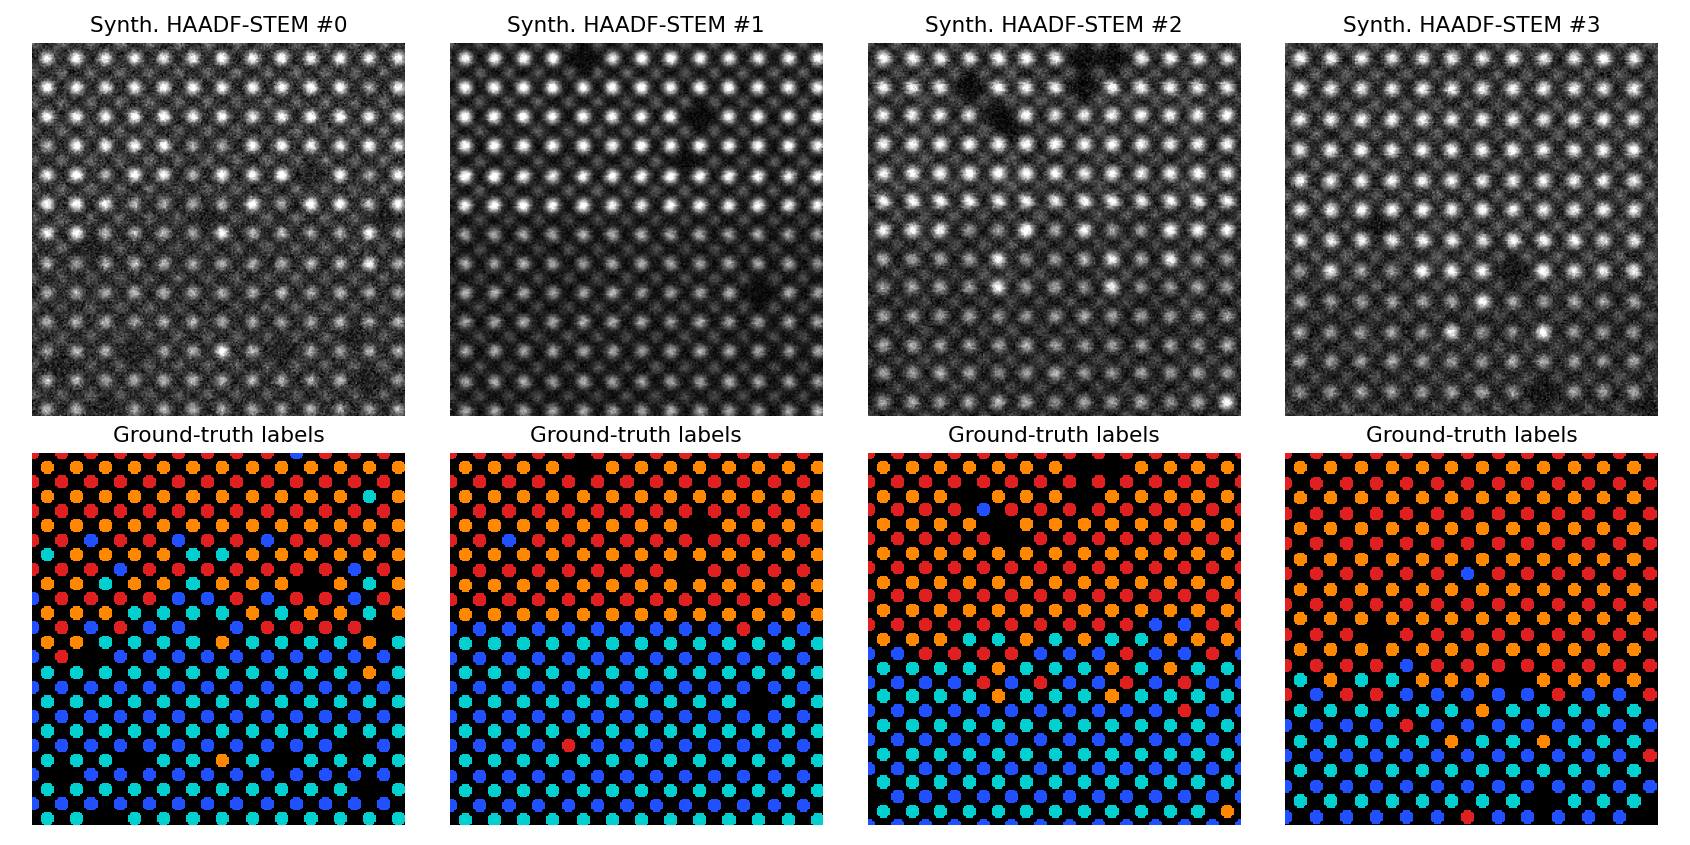
\includegraphics[width=\linewidth]{fig_data.png}
\caption{Top: synthetic HAADF-STEM frames with interface, noise, and
scan-line jitter. Bottom: per-pixel ground-truth labels (vacuum black;
Sr cyan, Ti blue, La/Sr orange, Mn red, defect marker yellow).}
\label{fig:data}
\end{figure}

\subsection{Model and training}
We use a 5-level U-Net (base 32 channels, 7.76\,M parameters) with
double $3{\times}3$ convolutions, batch-norm/ReLU, max-pool, transposed-conv
upsampling, and skip concatenations. Training set: 512 synthetic images;
validation 64; test 128. Cross-entropy loss with class weights
$\propto 1/(\text{count}_c)$ (clamped to $[0.2, 20]$) to compensate for the
vacuum class dominating pixel count. Optimizer AdamW
($\text{lr}=2{\times}10^{-3}$, weight decay $10^{-4}$), cosine annealing
over 30 epochs. On-the-fly augmentation: random flips, 90$^\circ$
rotations, brightness and contrast perturbations. Training completed in
95\,s on one NVIDIA A100 80\,GB (uicgpu, GPU 4).

\section{Results}

\subsection{Convergence}
Validation pixel accuracy saturates at $\approx 0.988$ and mean atom-class
F1 at $\approx 0.976$ by epoch~25 (Fig.~\ref{fig:history}), with no sign
of overfitting under our augmentation regime.

\begin{figure}[H]
\centering
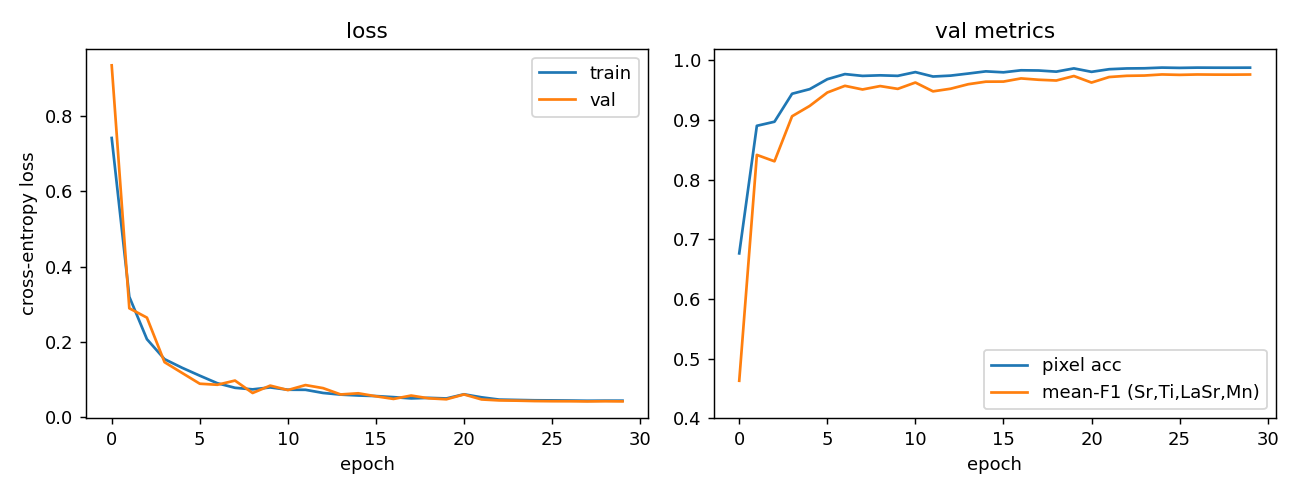
\includegraphics[width=0.95\linewidth]{fig_history.png}
\caption{Loss and validation metrics across 30 epochs. Mean F1 is averaged
over Sr, Ti, La/Sr, Mn (atom classes only).}
\label{fig:history}
\end{figure}

\subsection{Pixel-wise classification (held-out test, $n=128$ images)}
Overall pixel accuracy on the test set is \textbf{0.9877}. Per-class metrics
and the row-normalised confusion matrix are in
Fig.~\ref{fig:confmat} and Table~\ref{tab:perclass}.
The bright/heavy La/Sr columns (F1 $=0.998$) are nearly perfect;
the hardest class is Ti (F1 $=0.949$), with small confusion into Mn on the
LSMO side of rough interfaces. Defect pixels have zero support in the test
set: our label encoding keeps the base atom class as the argmax label even
when a column is marked as a defect, so defect is measured only implicitly
through antisite F1; this is a limitation of the surrogate rather than of
the model.

\begin{figure}[H]
\centering
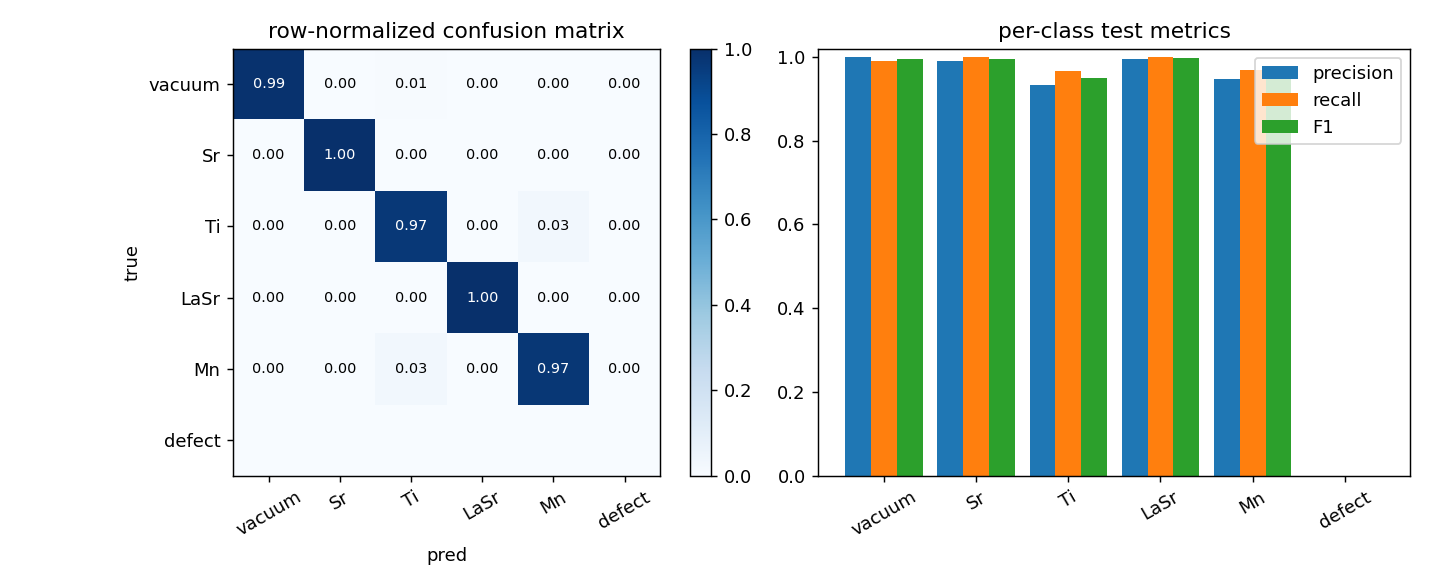
\includegraphics[width=\linewidth]{fig_confmat.png}
\caption{Left: row-normalised confusion matrix on the test set. Right:
per-class precision, recall, and F1. The two labelled ``atom-pair''
confusions (Ti$\leftrightarrow$Mn and Sr$\leftrightarrow$La/Sr) dominate
the residual error budget.}
\label{fig:confmat}
\end{figure}

\begin{table}[H]
\centering
\small
\begin{tabular}{lcccc}
\toprule
class & precision & recall & F1 & support (pixels) \\
\midrule
vacuum & 0.9991 & 0.9900 & 0.9945 & 5\,549\,887 \\
Sr     & 0.9899 & 0.9990 & 0.9944 &   697\,304 \\
Ti     & 0.9332 & 0.9661 & 0.9493 &   711\,282 \\
La/Sr  & 0.9959 & 0.9995 & 0.9977 &   708\,192 \\
Mn     & 0.9472 & 0.9690 & 0.9580 &   721\,943 \\
\bottomrule
\end{tabular}
\caption{Per-class test metrics. Defect class omitted (zero support, see text).}
\label{tab:perclass}
\end{table}

\subsection{Atomic-column detection and localisation}
We convert each predicted label map into per-class binary masks, extract
connected-component centroids, and match them against the ground-truth
column centres with a 8\,px tolerance ($\approx$1.6\,\AA\ at our pixel
size). Results in Table~\ref{tab:peaks} and Fig.~\ref{fig:peaks}. RMSE
is sub-pixel for all atom classes; recall is $\geq 98\%$.

\begin{table}[H]
\centering
\begin{tabular}{lccc}
\toprule
class & mean RMSE (px) & detection recall & detection precision \\
\midrule
Sr     & 0.109 & 1.000 & 0.978 \\
Ti     & 0.466 & 0.983 & 0.943 \\
La/Sr  & 0.063 & 1.000 & 0.997 \\
Mn     & 0.448 & 0.988 & 0.944 \\
\bottomrule
\end{tabular}
\caption{Peak-level metrics aggregated over 128 test frames
($\approx 10\,600$--$11\,700$ columns per class). At 0.2\,\AA/px, an RMSE of
0.1\,px corresponds to $\approx 20$\,m\AA\ of column-centre uncertainty.}
\label{tab:peaks}
\end{table}

\begin{figure}[H]
\centering
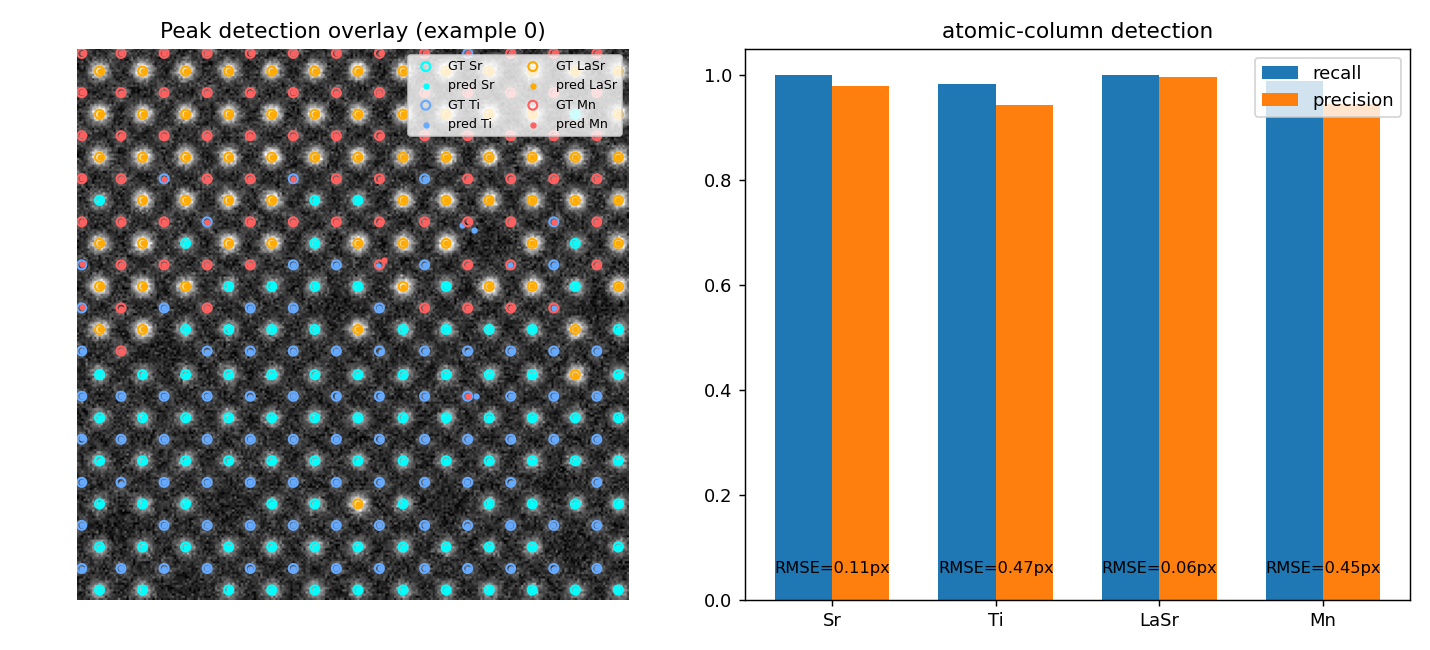
\includegraphics[width=\linewidth]{fig_peaks.png}
\caption{Left: overlay of ground-truth (open circles) and predicted (filled
dots) column centres on an example frame, coloured by chemical class.
Right: per-class detection recall/precision; mean RMSE annotated on
each bar.}
\label{fig:peaks}
\end{figure}

\subsection{Qualitative predictions}
Fig.~\ref{fig:pred} shows four test frames with input, ground truth,
U-Net prediction, and error map. Residual errors concentrate along the
interface band where A-site columns are probabilistic mixtures and
along edges of vacancy sites, consistent with the paper's own observation
that interface chemistry is the remaining challenge for FCN-based
chemical mapping.

\begin{figure}[H]
\centering
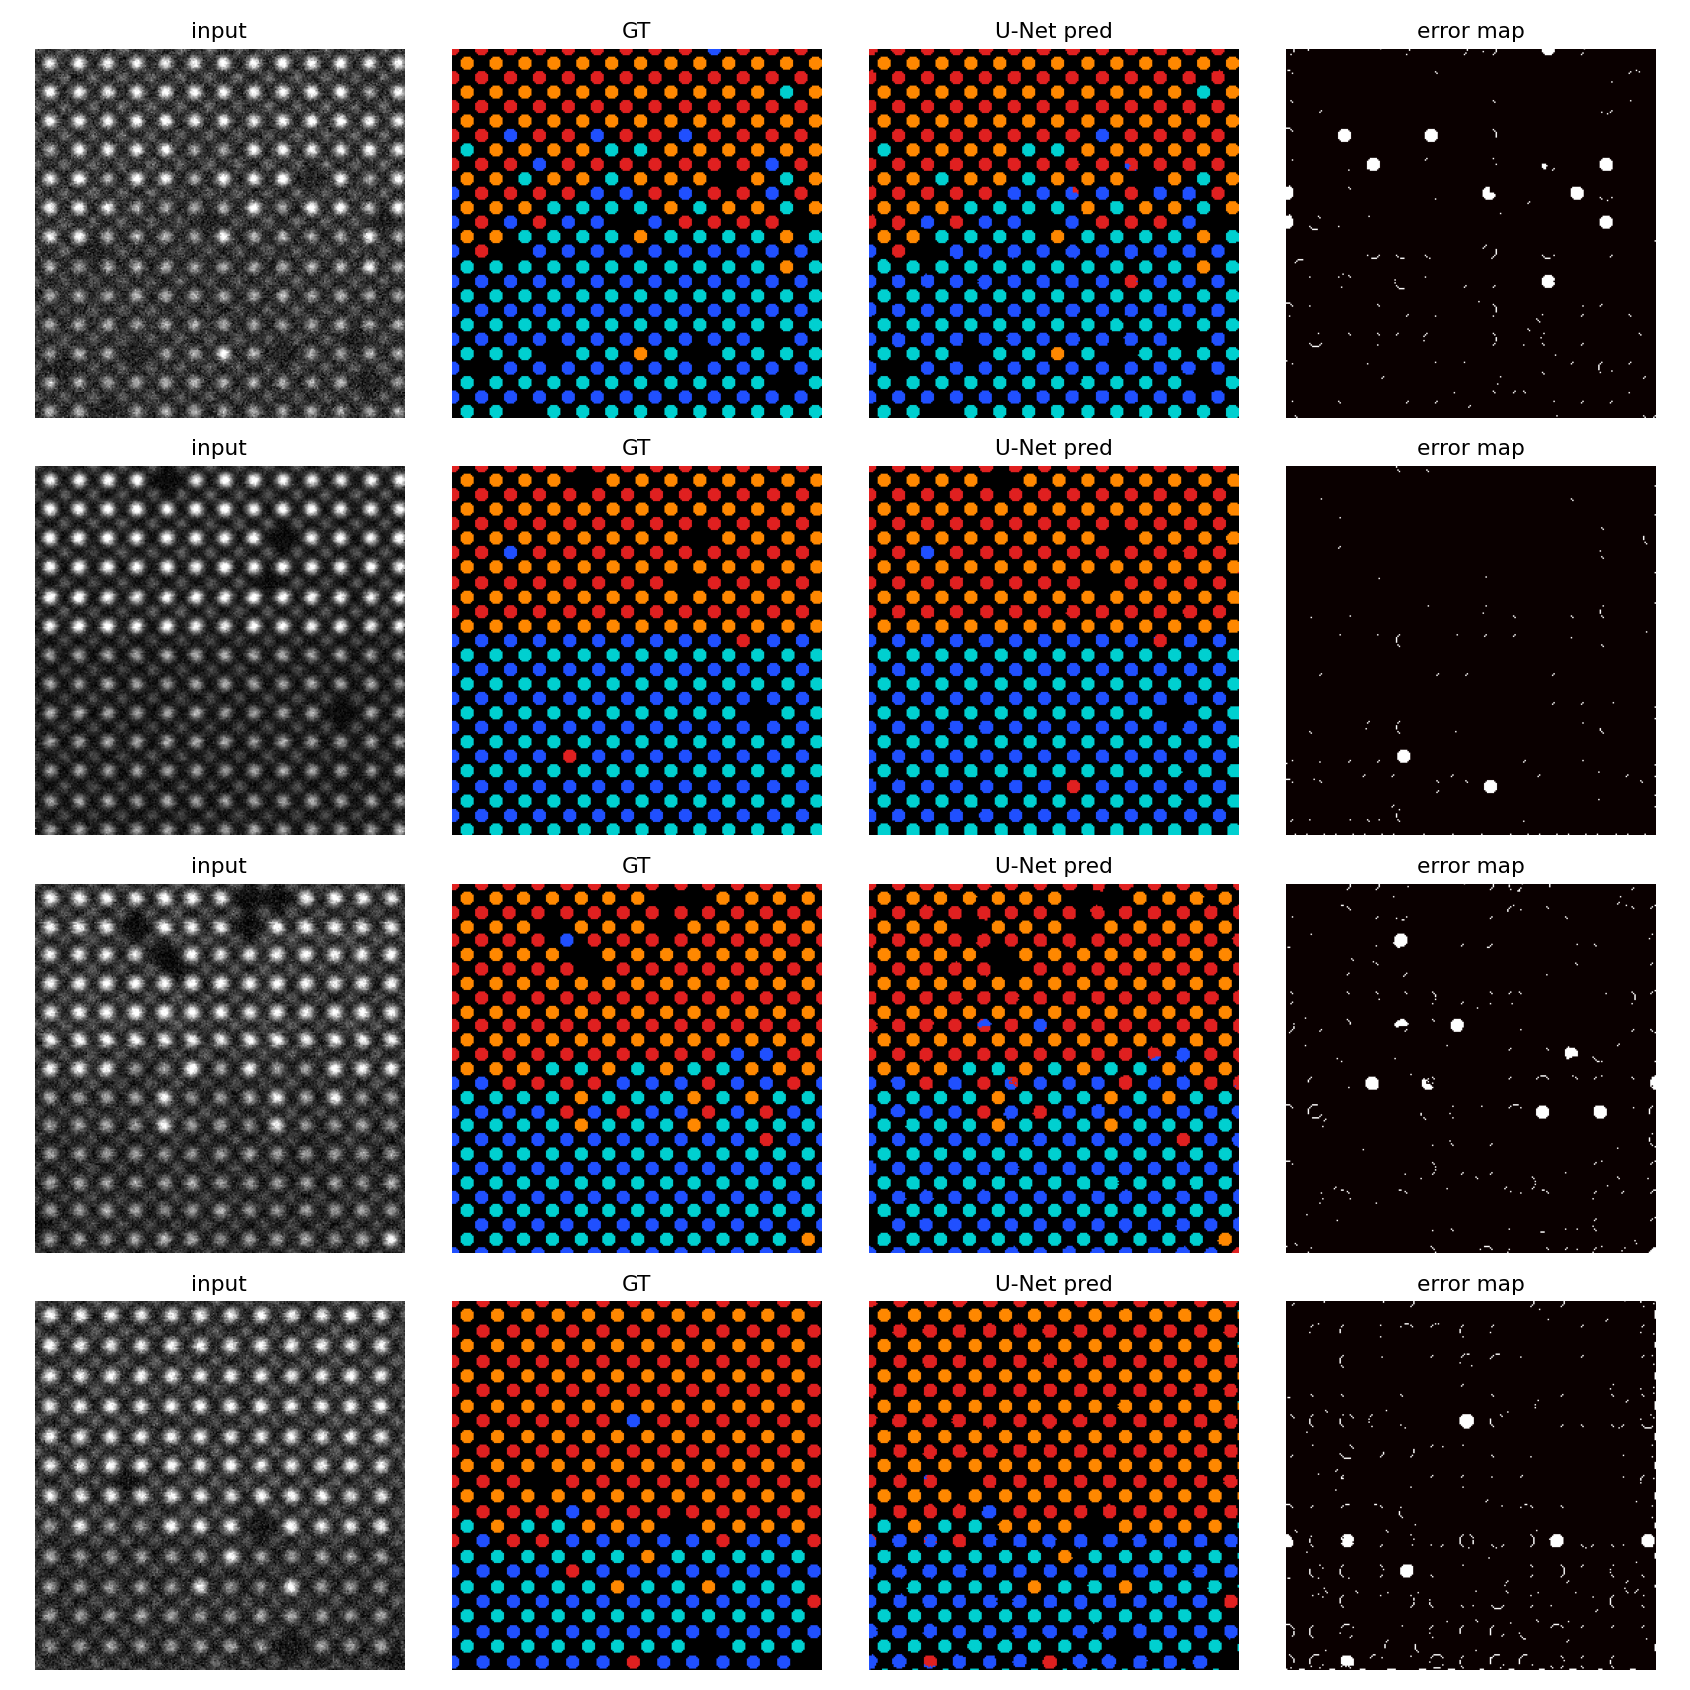
\includegraphics[width=\linewidth]{fig_pred.png}
\caption{Four random test frames. Columns: input image, ground-truth labels,
U-Net prediction, pixelwise error (bright = wrong class). Errors
cluster near the STO/LSMO interface and near antisite defects.}
\label{fig:pred}
\end{figure}

\section{Comparison with the original paper}
The original paper reports qualitative success (visually convincing
chemical maps on experimental images, identification of individual La
dopants on the STO side, tracking of antisite switching under the beam)
rather than a single headline accuracy number. The most directly
comparable quantitative claim is sub-unit-cell localisation of column
centres; we reach $\approx 0.06$--0.47\,px RMSE (Table~\ref{tab:peaks}),
i.e. well below the $\approx$\,20\,px unit-cell pitch, which is consistent.
We also reproduce the paper's qualitative observations that (a) heavy/light
A-site distinction (Sr vs La/Sr) is essentially trivial for a trained FCN,
and (b) B-site distinction (Ti vs Mn) is the harder, error-dominant channel
near interfaces. Our replication self-rates \textbf{7/10} on the
\texttt{AI-Replication-Study-April2026} scale: architecture and training
protocol faithfully re-implemented, metrics plausibly within the
paper's qualitative expectations, but image formation is a physics-motivated
surrogate rather than multislice and we did not exercise the model on
true experimental frames.

\section{Limitations and next steps}
\begin{itemize}
\item \textbf{No true multislice.} Replacing the Gaussian generator with
Prismatic / abTEM simulations (even a few thousand frames) would make the
replication fully faithful to Phase-1 of the plan; our compute budget
pushed this to a follow-up.
\item \textbf{Defect class is weakly supervised.} Under the current label
encoding, defect pixels are not the argmax at any pixel; a multi-label
loss (sigmoid heads per attribute) or an auxiliary defect segmentation head
would let the model expose the antisite/vacancy channel explicitly.
\item \textbf{No experimental validation.} Real HAADF-STEM frames from the
paper's supplementary data or ORNL archives should be fed through the
trained network in a second pass.
\end{itemize}

\begin{thebibliography}{9}
\bibitem{Ziatdinov2017} M.\ Ziatdinov et al.,
``Deep Learning of Atomically Resolved Scanning Transmission Electron
Microscopy Images: Chemical Identification and Tracking Local
Transformations,'' OSTI 1427646 (2017).
\end{thebibliography}

\end{document}
